\documentclass[11pt]{article}

\usepackage{fullpage} % Use the full page
\usepackage{color}
\usepackage{tikz}
\usepackage{matlab-prettifier} % Matlab
\setlength\parindent{0pt} % No indentation


% Headers
\usepackage{fancyhdr}
\setlength{\headheight}{15.2pt}
\pagestyle{fancy}
\setlength\headsep{30pt}
\lhead{Youssef Beltagy and Samuel Hunter}   					%  Your name on the left header.
\chead{\textsc{Lab 3}}			%  Title in the center.
\rhead{\today}							%  Date on the right header.

% Matlab blocks
\lstset{
  style              = Matlab-editor,
  basicstyle         = \mlttfamily,
  mlshowsectionrules = true,
  escapeinside={//}{\^^M},
}

% Cover Page Settings
\title{
    \textsc{Lab 3 Report: Fourier Series and Gibbs Phenomenon}
}

\author{
    \Large{Youssef Beltagy and Samuel Hunter} \\
    \large \textsc{AUT21 BEE 235}
}

\date{\today}



%--------------------------------------------
%%%%%%%%%%%%%%%%%%%%%%%%%%%%%%%%%%%%%%%%%%%%%%%%%%%%
% END OF THE PREAMBLE AND BEGINNING OF THE ACTUAL DOCUMENT
%%%%%%%%%%%%%%%%%%%%%%%%%%%%%%%%%%%%%%%%%%%%%%%%%%%%
%--------------------------------------------

\begin{document}


\maketitle % Make the cover page
\pagebreak


\section{Abstract}

We experiment with fourier series signal synthesis and
observe the limitations of this technique.
% =================================================
% PART 1
% =================================================
\section{Part 1 --- Description}


% =================================================
% PART 2
% =================================================
\pagebreak
\section{Part 2 --- Fourier Series Approximation of a Square Wave}

In this section, we synthesized a square wave signal using a fourier series.
When the number of coefficients is low, the synthesized signal displays the Gibbs
phenomenon where the signal overshoots and undershoots at sharp transitions.

\subsection{C\_k Phase and Magnitude}

We generated and plotted the C\_k coefficients of the fourier series
we used to synthesize the square wave.\\

Below you can see the magnitudes and phases of the coefficients.

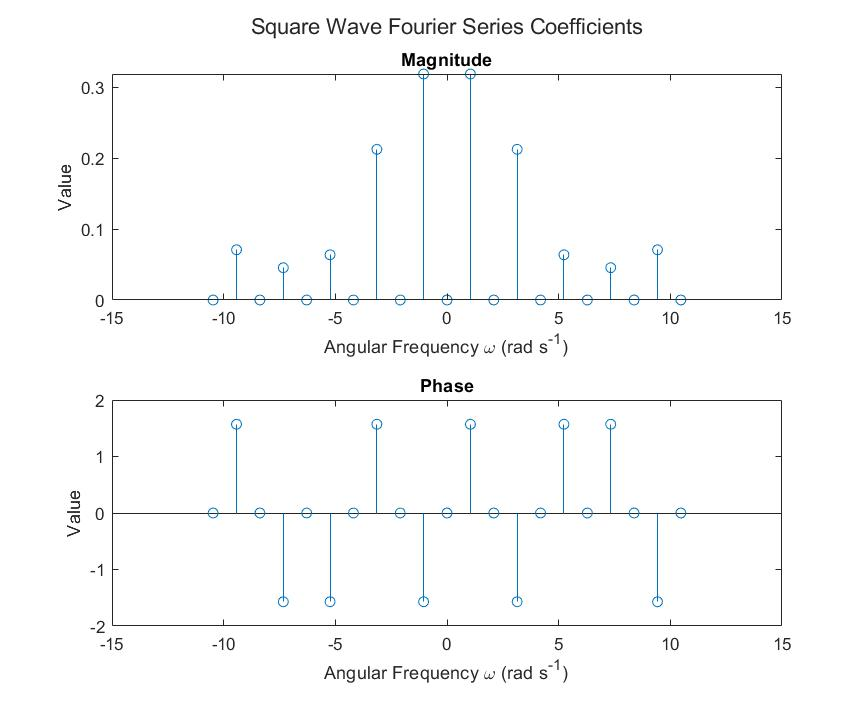
\includegraphics[width=\textwidth]{ck_values.png}

\lstinputlisting{gibbs.m}

\subsection{Square Wave Synthesis}

We developed a function that generates an approximation of a square wave
given the time of the signal and the K\_{max} of the coefficients.

\lstinputlisting{squarewave.m}

\subsection{Square Wave Plots}

We plotted the output from our synthesizing function.

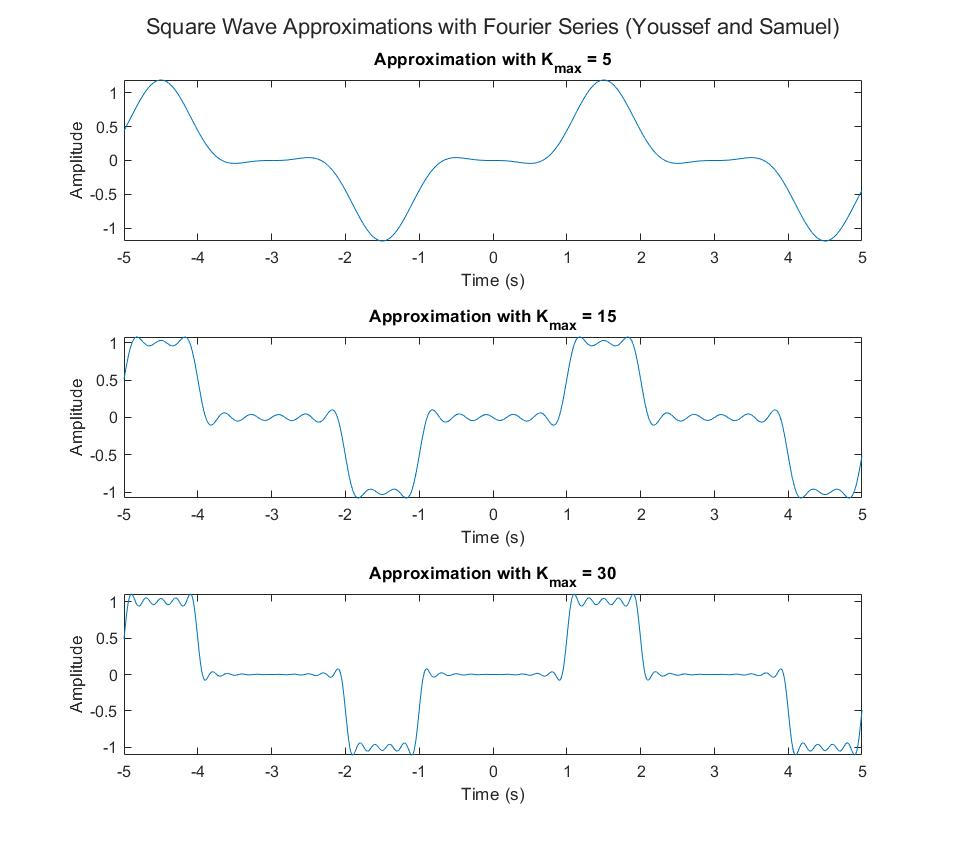
\includegraphics[width=\textwidth]{squarewaves.png}

\lstinputlisting{squarewave_plot.m}

\subsection{Gibbs Phenomenon}

The plots didn't demonstrate the phenomenon enough,
so we wrote a script to generate a video of synthesized signal
as k\_{max} increases.

\lstinputlisting{squarewave_video.m}

When K\_{max} is less than 500, the Gibbs phenomenon is clear.
The signal rings (overshoots and undershoots) at sharp transitions.\\

Between K\_{max} = 400 and K\_{max} = 500, the ringing decreases.
When K\_{max} rises above 500, the Gibbs phenomenon disappears.
After that it appears again; then it disappears again; 
then it appears again, and the process repeats.

\section{Conclusion}

In this lab, we synthesized a square wave using 
fourier series and observed the Gibbs phenomenon.
\end{document}
